The initial step in solving the task was to read up on the technical details on the AT32AP7000 \cite{ap7000} microcontroller, the STK1000 development-board and the the AVR32 instruction set \cite[Section 9]{avr32} in order to figure out how to actually solve the assignment. Then a plan of five subsequent steps was made.

\begin{enumerate}
\item Activate LEDs
\item Read button states
\item Make use of interrupts
\item Optimize for energy efficiency
\item Add additional functionality if time allows
\end{enumerate}

The reason for splitting up the assignment into smaller parts was due to debugging and ensuring some measure of incremental success, instead of attempting to solve the whole assignment in one go and ending up debugging for weeks.
\subsection{Jumper and cable configuration}


\begin{itemize}
\item The LED’s were connected to PIOC by a flat-cable from GPIO pins 16-23(J3) to the LED-pins(J15) on the STK1000 board \cite[section~2.4.1]{compendium}. 
\item The buttons were connected to PIOB by flat-cable from GPIO pins 0-7(J1) to the SWITCH-pins(J25) on the STK1000 board \cite[section~2.4.1]{compendium}.
\item On the AT32AP7000 we set the jumpers SW6 and SW4 to GPIO(so that PIOC and PIOB would be connected to GPIO)\cite[table~2.3]{compendium}.
\end{itemize}

\subsection{Using the debugger}

Setting up and using the debugger was crucial to our success. We got the debugger up during our first visit to the lab. In order to use the gdb debugger tool on the microcontroller, we had to set up a proxy, as well as use avr32s own version of gdb. The command given in the compendium\cite{compendium} gave us the following error: “Failed to look up the host localhost: 
Unknown server error“. This was solved by a quick google, which linked us to a thread at avrfreaks\cite{gdbforum} where someone had the same problems. It turns out that the command worked when run with no arguments, and we learned that the port 4711 was chosen by default. Therefore we ended up connecting the debugger to the microcontroller through JTAGICE mkII in the following steps:\\

\begin{verbatim}
$ avr32gdbproxy
$ avr32-gdb
(gdb) target remote:4711
\end{verbatim}

Because the proxy had to keep running, the second and third command were run in a different terminal window. We could have launched the proxy in the background with an ampersand, but we would then miss out on error messages and the like. 

The debugger was used by running the current code one instruction at a time with the “si” command and reading the register-values on each iteration with the “regs”, checking if the values were correct and then changing the code accordingly. Commands to set specific registers, or use breakpoints were not necessary for us during this assignment.
\subsection{LEDs}

As mentioned above, the first goal was to simply light up the LEDs. We used the value 0b11111111 to target all the LEDs, and started by writing the value to the Pin Enable Register (PER) and Output Enable Register (OER) of PIOC where the LEDs were connected. Then we wrote the value 0b10101010 to the Set Output Data Register (SODR) to turn every other LED on. The reason for using such a pattern was to make sure it was easy to recognize that is was our code that doing the job and not random noise. After this the program would just continue in an infinite loop.

We experienced a lot of random lights turning on at first, but solved this using the debugger, and found the problem to probably be loading of wrong pointers.
\subsection{Buttons}

With the LEDs up and running, the next step was to get the buttons under control. We used the value 0b11111111 to target all the buttons, and started by writing the value to the Pin Enable Register (PER) and Pull-Up Enable Register (PUER) of PIOB where the buttons were connected. Now in the infinite loop, we read the Pin Data Status Register (PDSR) and invert it to get the status of the buttons where a one means that the button is down. We also masked this value against 0b11111111 to remove any unwanted noise. Then all LEDs were cleared before writing the button statuses to to SODR to light the LEDs over the pressed buttons.

With the ability to read the buttons it was time to make them move the light. By masking the buttons statuses to find which buttons are pressed we branched to different subroutines that updates a common registry containing one and only one 1 by either shifting it left or right, and then updating the LEDs. Special checks was added so that the light would wrap around. Since each iteration of the main loop is so quick, the light appeared to move at random during normal operation, but we could see that it was working correctly with the debugger and thought implementing interrupts would fix it.
\subsection{Interrupts}

\begin{figure}
  \centering
    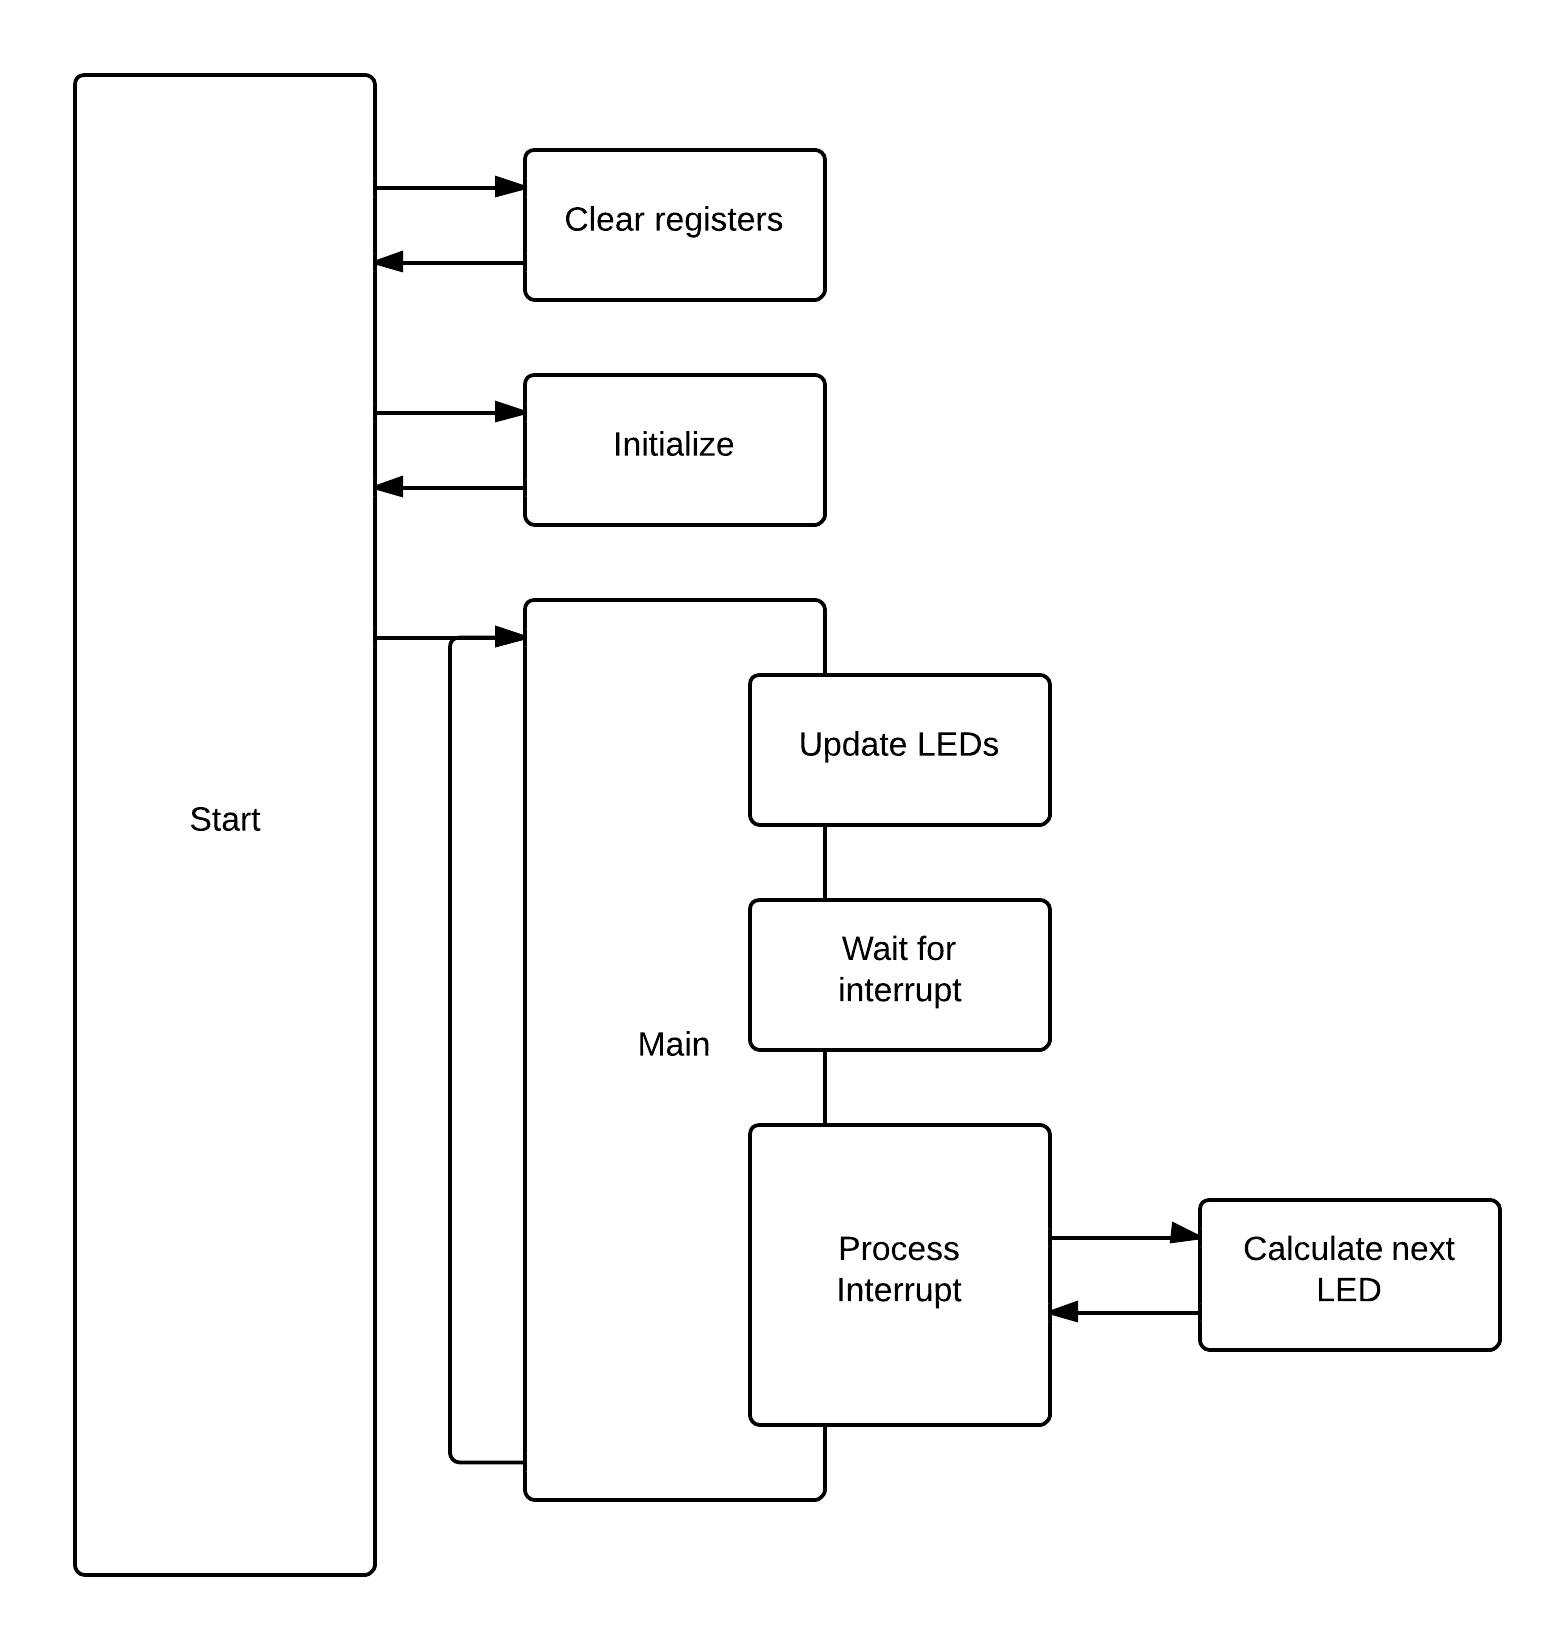
\includegraphics[width=0.4\textheight]{mainstructure}
 \caption{Structure of initialization and main loop}
 \label{mainstruct}
\end{figure}

\begin{figure}
  \centering
    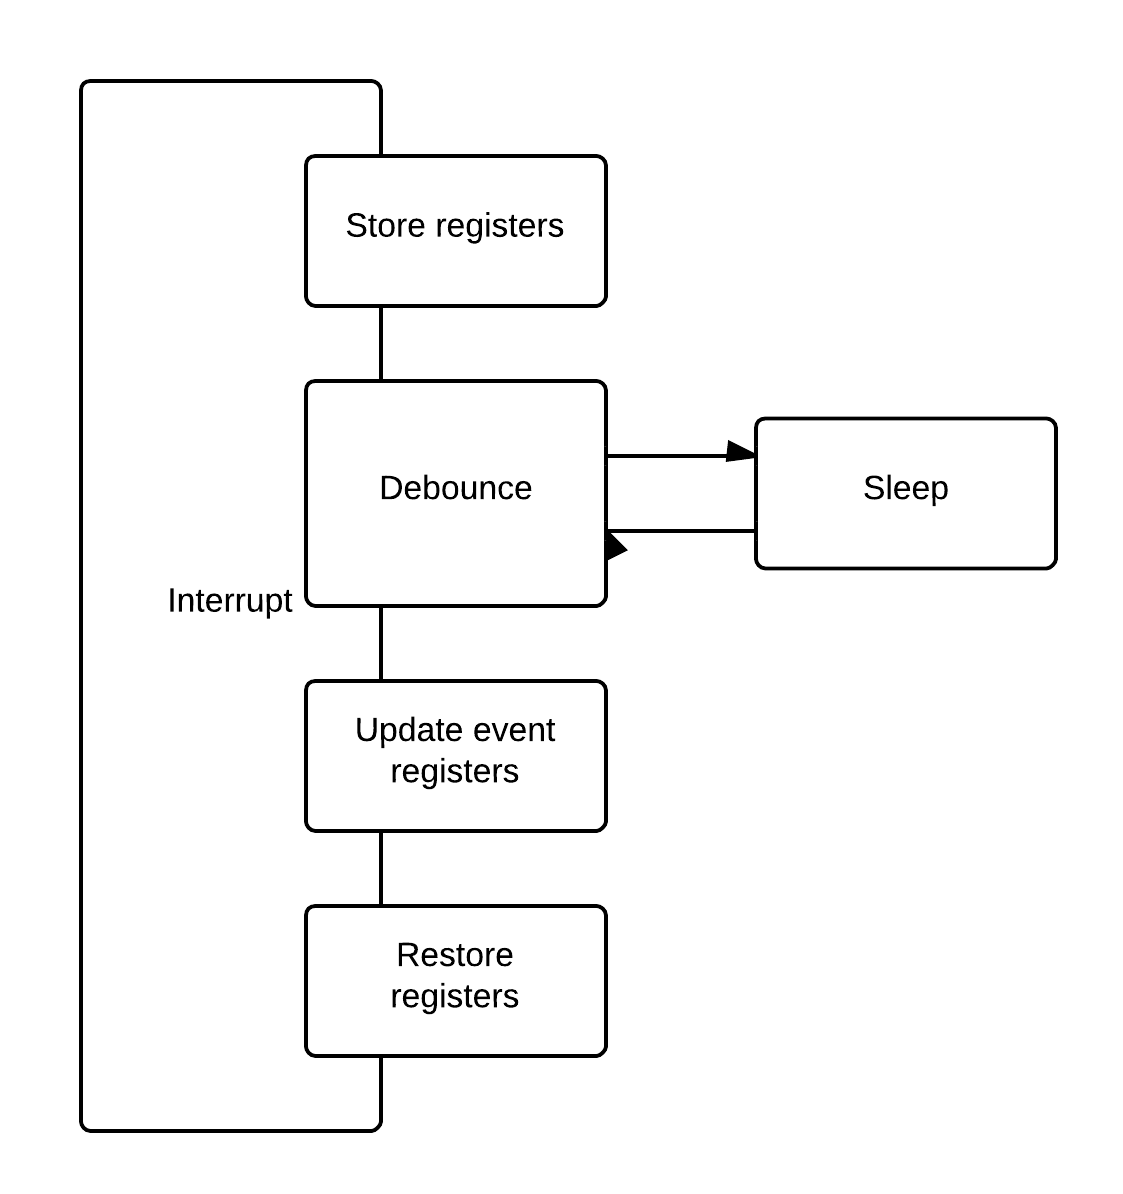
\includegraphics[height=0.4\textheight]{Interrupt}
  \caption{Structure of interrupt handler}
  \label{interruptstruct}
\end{figure}


Now that the buttons and LEDs were operating correctly, the next step was to implement interrupt handling by following the procedure in the compendium \cite[Section 2.5.2]{compendium}.

We started by creating the interrupt routine which stores the button states and event states to some specified registers which the main loop would then read. Except from using a special return command, this is just like a normal routine, but since the interrupt can occur at any time, all registers that is to be modified by the routine must first be stored in the memory, and then restored afterwards. A practical way to achieve this is by using a stack. This was accomplished by initializing the Stack Pointer (SP) to the built-in assembler address \_stack, and using load and store instructions which update the SP. Structure of the main routine is shown in figure \ref{mainstruct}, and structure of the interrupt routine is shown in figure \ref{interruptstruct}.

Once the routine was functional, the interrupts had to be set up. To accomplish this, the Input Enable Register (IER) is set for the pins connected to the buttons, and the Input Disable Register (IDR) is set for all other pins on PIOB to prevent unwanted events to be triggered by noise. Afterwards the Exception Vector Base Address (EVBA) is set to zero for simplicity, and an autovector of the exception’s address and priority zero is stored in the interrupt controller’s Interrupt Priority Register 14 (IPR14), which corresponds to PIOB. Finally, the Global Interrupt Mask (GM) status register is cleared.

The interrupt handler was now more or less complete. However, each press generated several events due to bouncing, and the program did not distinguish between between presses and releases because we used the data from the Interrupt Status Register (ISR). Therefore, debouncing was added by waiting for a short while after an interrupt before processing the event. This was accomplished by decrementing a large number (we used 1000) down one by one to 0. Finally, a check for whether the button is now pressed or released was added by reading the PDSR as in the previous section.

\subsection{Energy optimization}

After all the main functionality was in place, it was time to optimize the code where possible to conserve energy. As the program is only supposed to react to interrupts, the first and most obvious step was to put the microcontroller into a sleep state while waiting for them instead of running in an infinite loop. This allows nearly all parts of the board to be shut down for most of the time, which conserves huge amounts of energy.

Some more energy can be saved by making the code more efficient, i.e. execute faster, which allows the board to re-enter a sleep state earlier. Therefore, the number of instruction was reduced where possible, although there were not many places this could be performed. Branches were also exchanged with conditional instructions where possible, as clearing the whole seven step pipeline can take a lot of time. These actions were taken somewhat into account from the beginning of the assignment, but a second pass did not hurt.
\subsection{Additional functionality}

A little extra time allowed us to implement some additional functionality. Specifically, switch 5 (SW5) will make the LEDs flash to the right for a few seconds, while switch 7 (SW7) will make the LEDs flash to the left for a few seconds. Additionally, switch 6 (SW6) will make the LEDs flash outwards in both directions from the currently lit LED.


\subsection{Tools}


\begin{itemize}
\item GitHub for handling version control
\item Vim as main code-editor
\item Google Docs for report collaboration
\item \LaTeX for report markup
\item JTAGICE mkII for connecting the computer to the board
\item avr32gdbproxy for connecting to JTAGICE mkII
\item avr32-gdb for connecting to the board, allowing us to debug the code
\end{itemize}

